\documentclass[11pt,a4paper]{article}

% -------------------------------------------------------------
% 1. TYPOGRAPHY & FONT SETUP (TIMES NEW ROMAN)
% -------------------------------------------------------------
\usepackage[T1]{fontenc}
\usepackage[utf8]{inputenc}
\usepackage{newtxtext}
\usepackage{newtxmath}

% Page Geometry (Structured one-section-per-page layout, 6 pages)
\usepackage[top=0.75in, bottom=0.75in, left=0.82in, right=0.82in]{geometry}
\usepackage{setspace}
\setstretch{1.12}

% Utilities
\usepackage{graphicx}
\usepackage{float}
\usepackage{booktabs}
\usepackage{enumitem}
\usepackage{titlesec}
\usepackage{caption}
\usepackage{hyperref}
\usepackage{fancyhdr}
\usepackage{xcolor}

% Balanced figure spacing
\setlength{\textfloatsep}{7pt plus 1pt minus 1pt}
\setlength{\intextsep}{7pt plus 1pt minus 1pt}
\setlength{\abovecaptionskip}{4pt}
\setlength{\belowcaptionskip}{4pt}

% IBM Brand Palette
\definecolor{ibmblue}{RGB}{5, 47, 173}
\definecolor{charcoal}{RGB}{35, 35, 35}
\definecolor{rulecolor}{RGB}{200, 205, 215}

% -------------------------------------------------------------
% 2. HEADINGS, HEADERS & CAPTIONS
% -------------------------------------------------------------
\titleformat{\section}
  {\fontsize{12pt}{15pt}\selectfont\bfseries\color{ibmblue}}{\thesection}{0.8em}{}
\titleformat{\subsection}
  {\fontsize{10.8pt}{14pt}\selectfont\bfseries\color{charcoal}}{\thesubsection}{0.8em}{}
\titleformat{\subsubsection}
  {\fontsize{10.2pt}{13pt}\selectfont\bfseries\itshape\color{charcoal}}{\thesubsubsection}{0.8em}{}

% Generous breathing room above headings
\titlespacing*{\section}{0pt}{11pt plus 2pt minus 1pt}{4pt}
\titlespacing*{\subsection}{0pt}{8pt plus 2pt minus 1pt}{3pt}
\titlespacing*{\subsubsection}{0pt}{5pt plus 1pt minus 1pt}{2pt}

\captionsetup{
    font={small},
    labelfont={bf},
    labelsep=period,
    skip=3pt
}

% Running Header & Footer
\pagestyle{fancy}
\fancyhf{}
\lhead{\small \textcolor{gray}{\textbf{AICTE--IBM SkillsBuild Capstone Report}}}
\rhead{\small \textcolor{gray}{Internship ID: \textbf{IBMUEDA0483}}}
\cfoot{\small \thepage}
\renewcommand{\headrulewidth}{0.4pt}

% Hyperlinks
\hypersetup{
    colorlinks=true,
    linkcolor=ibmblue,
    citecolor=ibmblue,
    urlcolor=ibmblue
}

% Natural, breathable lists
\setlist{topsep=2.5pt, itemsep=3pt, parsep=0pt}

% -------------------------------------------------------------
% 3. DOCUMENT BODY
% -------------------------------------------------------------
\begin{document}

% =============================================================
% PAGE 1: EXECUTIVE FRAMING, PROBLEM & UN SDGS
% =============================================================

\begin{center}
    {\fontsize{18pt}{22pt}\selectfont \textbf{Credit Risk Assessment \& Automated Loan Underwriting Engine}}\\[0.20cm]
    {\fontsize{11pt}{13.5pt}\selectfont \textbf{AICTE--IBM SkillsBuild Data Analytics with AI Internship 2026}}\\[0.10cm]
    {\fontsize{10pt}{12pt}\selectfont Machine Learning Pipeline with Feature Engineering and Descriptive Fairness Auditing}\\[0.28cm]
    
    {\fontsize{10pt}{12pt}\selectfont \textbf{Srijan Das} \quad | \quad \textbf{Internship ID:} IBMUEDA0483} \\
    {\fontsize{9.5pt}{11.5pt}\selectfont Department of Computer Science \& Engineering} \\
    {\fontsize{9.5pt}{11.5pt}\selectfont Cooch Behar Government Engineering College (CGEC), West Bengal} \\
    {\fontsize{9pt}{11pt}\selectfont Email: \href{mailto:srijandas9073@gmail.com}{srijandas9073@gmail.com} \quad | \quad LinkedIn: \href{https://www.linkedin.com/in/srijandas2099}{linkedin.com/in/srijandas2099}} \\[0.12cm]
    {\fontsize{9.5pt}{11.5pt}\selectfont September 2026}
\end{center}

\noindent\textcolor{rulecolor}{\rule{\textwidth}{0.6pt}}

\begin{quote}
\small \textbf{Abstract}---Manual loan underwriting varies across individual branch reviewers and creates processing bottlenecks during peak application cycles. This project evaluates whether a structured machine learning pipeline can provide consistent first-pass approval recommendations using 614 historical applicant records from the benchmark Kaggle Loan Prediction dataset. The workflow integrates domain feature engineering (Total Income, Debt-to-Income, and estimated EMI) with median imputation fitted strictly within cross-validation training folds. A regularized Random Forest classifier achieves a \textbf{74.7\% ($\pm$ 5.1\%) 5-fold cross-validation accuracy} (\textbf{+6.0 percentage points} over the 68.7\% majority-class baseline), an \textbf{81.3\% holdout test accuracy}, an \textbf{84.7\% approval recall} (72 of 85 approved cases identified), and an \textbf{0.85 ROC-AUC score}. In alignment with \textbf{UN SDG 8} and \textbf{UN SDG 10}, demographic attributes (\texttt{Gender}) are omitted from model features, and a descriptive check reports a historical female-to-male approval-rate ratio of 0.966.
\end{quote}

\noindent\textcolor{rulecolor}{\rule{\textwidth}{0.6pt}}

\section{Introduction \& Problem Definition}
Manual retail underwriting often introduces operational variance across loan officers, creating turnaround delays for creditworthy borrowers while leaving institutions vulnerable to default risks.

This project builds an automated decision-support pipeline to:
\vspace{0.15cm}

\begin{itemize}
    \item Clean and profile 614 applicant records from a benchmark retail lending dataset.
    \item Identify empirical default drivers through Exploratory Data Analysis (EDA).
    \item Train an ensemble Scikit-Learn pipeline that eliminates imputation data leakage.
    \item Deploy an interactive Streamlit dashboard for real-time applicant risk scoring.
\end{itemize}

\subsection{UN Sustainable Development Goals (UN SDGs) Alignment}
\vspace{0.15cm}

\begin{itemize}
    \item \textbf{UN SDG 8 (Decent Work \& Economic Growth):} Streamlining initial underwriting reduces application turnaround latency, supporting financial access for eligible households and micro-enterprises.
    \item \textbf{UN SDG 10 (Reduced Inequalities via Fairness Auditing):} Demographic variables were audited for historical rate disparities (female-to-male approval ratio = 0.966, meeting the Four-Fifths regulatory benchmark). To eliminate direct disparate treatment, \texttt{Gender} was excluded from the model feature matrix. \textit{Note: This comparison serves as a historical baseline check; production implementations would require continuous subgroup error-rate tracking.}
\end{itemize}

\clearpage

% =============================================================
% PAGE 2: DATASET ARCHITECTURE & PREPROCESSING
% =============================================================

\section{Dataset Architecture \& Preprocessing Pipeline}
The system utilizes the \textbf{Kaggle Loan Prediction Problem Dataset}, containing 614 applicant records across 12 financial and demographic attributes.

\begin{figure}[H]
    \centering
    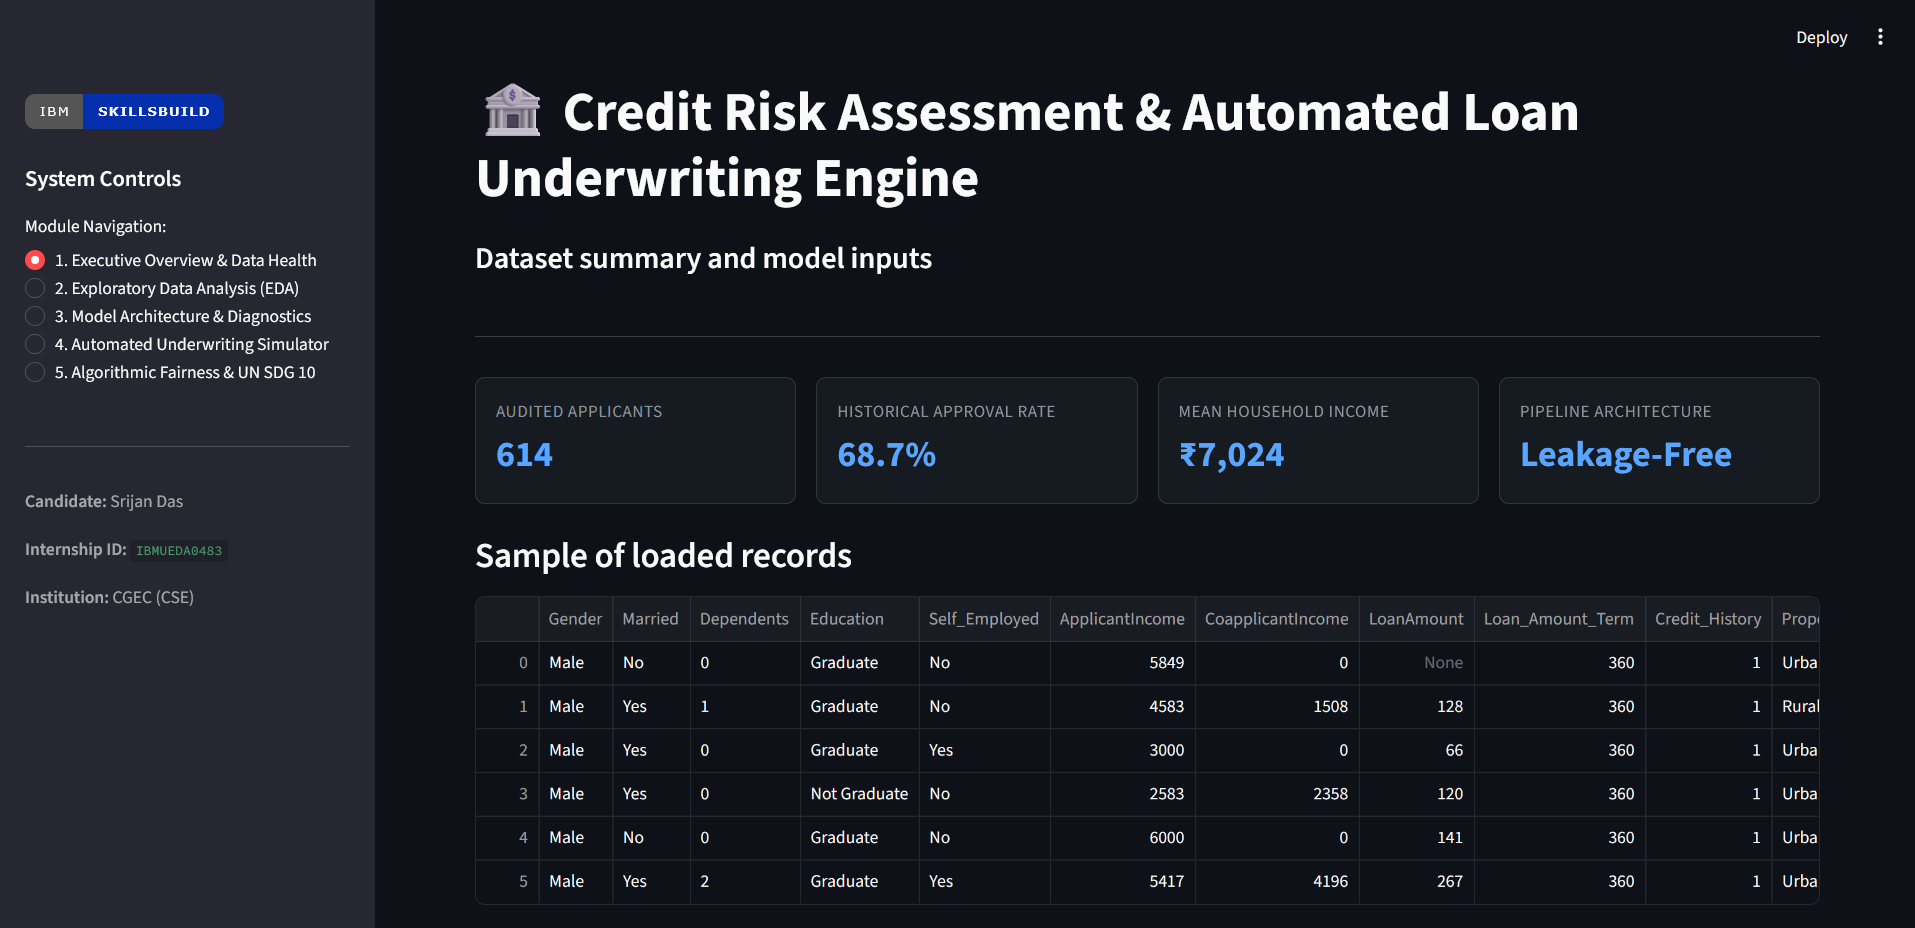
\includegraphics[width=0.78\linewidth]{fig1_overview.png}
    \caption{Executive Overview Module displaying dataset metrics, record counts, and loaded data sample.}
    \label{fig:overview}
\end{figure}

\subsection{Data Cleaning \& Pipeline Imputation}
Inspection revealed missing values across continuous and categorical fields. To eliminate data leakage, imputation is handled strictly inside a Scikit-Learn \texttt{Pipeline} fitted solely on training splits:

\vspace{0.15cm}

\begin{itemize}
    \item \textbf{Integrated Imputation:} Missing values in numerical features (\texttt{LoanAmount}, \texttt{Loan\_Amount\_Term}) and encoded binary indicators (\texttt{Credit\_History}, \texttt{Married}) receive pipeline-fitted median imputation.
    \item \textbf{Feature Pruning:} Low-variance attributes (\texttt{Self\_Employed}, \texttt{Dependents}) and protected attributes (\texttt{Gender}) were excluded from the model matrix to reduce noise and prevent demographic bias.
\end{itemize}

\begin{figure}[H]
    \centering
    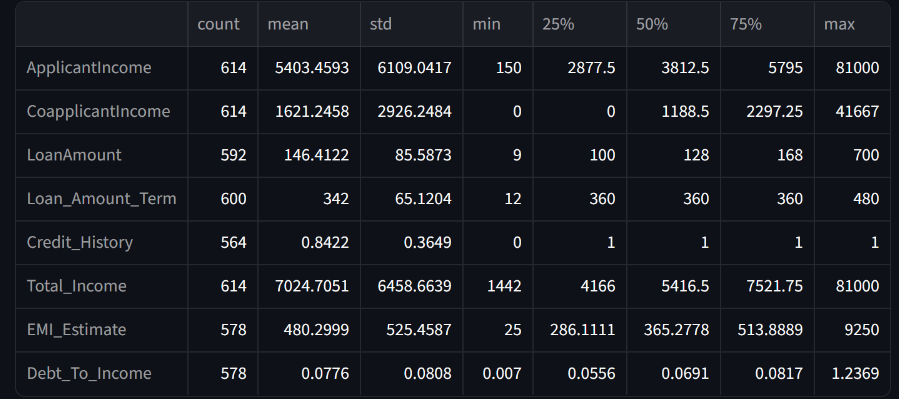
\includegraphics[width=0.76\linewidth]{fig1_overview2.png}
    \caption{Summary Statistics for the Cleaned Feature Set.}
    \label{fig:stats}
\end{figure}

\subsection{Feature Engineering}
These three engineered financial indicators provide the model with direct readouts of debt-servicing capacity rather than relying solely on raw gross income:

\vspace{0.15cm}

\begin{enumerate}
    \item $\text{Total Income} = \text{ApplicantIncome} + \text{CoapplicantIncome}$
    \item $\text{Estimated Monthly Obligation (EMI)} = \frac{\text{LoanAmount} \times 1000}{\text{Loan\_Amount\_Term}}$
    \item $\text{Debt-to-Income (DTI)} = \frac{\text{Estimated EMI}}{\text{Total Income} + \epsilon}$
\end{enumerate}

\clearpage

% =============================================================
% PAGE 3: EXPLORATORY DATA ANALYSIS (EDA)
% =============================================================

\section{Exploratory Data Analysis (EDA) \& Risk Discovery}
Exploratory analysis evaluated how financial features and property locations correlate with historical loan outcomes.

\begin{figure}[H]
    \centering
    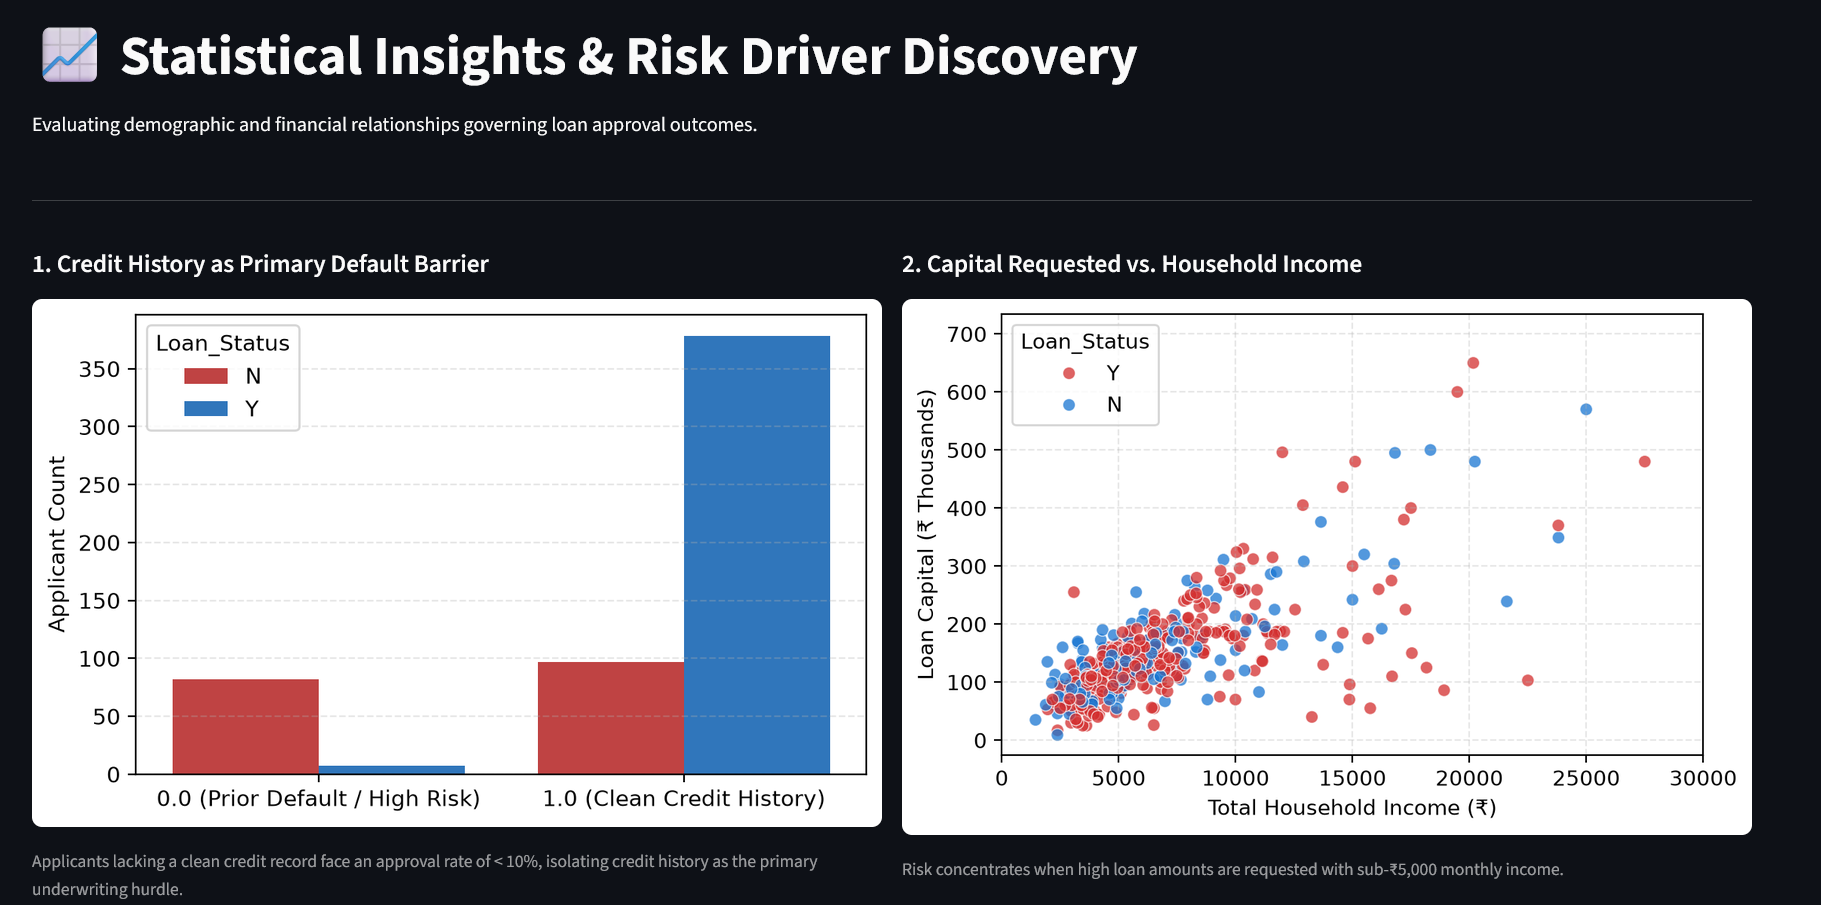
\includegraphics[width=0.78\linewidth]{fig2_eda.png}
    \caption{Exploratory Risk Analysis: (Left) Credit History approval barrier; (Right) Household Income vs. Requested Capital.}
    \label{fig:eda}
\end{figure}

\subsection{Key Analytical Insights}
\begin{itemize}
    \item \textbf{Credit History as Primary Hurdle:} As shown in Figure~\ref{fig:eda} (Left), applicants with a clean credit record (\texttt{1.0}) exhibit an approval rate exceeding \textbf{79\%}, compared to below \textbf{10\%} for applicants with adverse credit records (\texttt{0.0}).
    \item \textbf{Loan Capital vs. Income Distribution:} Figure~\ref{fig:eda} (Right) shows that requested loan capital scales moderately with household income, though variance widens among higher earners. Risk of default occurs across all income tiers rather than clustering solely in low-income segments.
\end{itemize}

\begin{figure}[H]
    \centering
    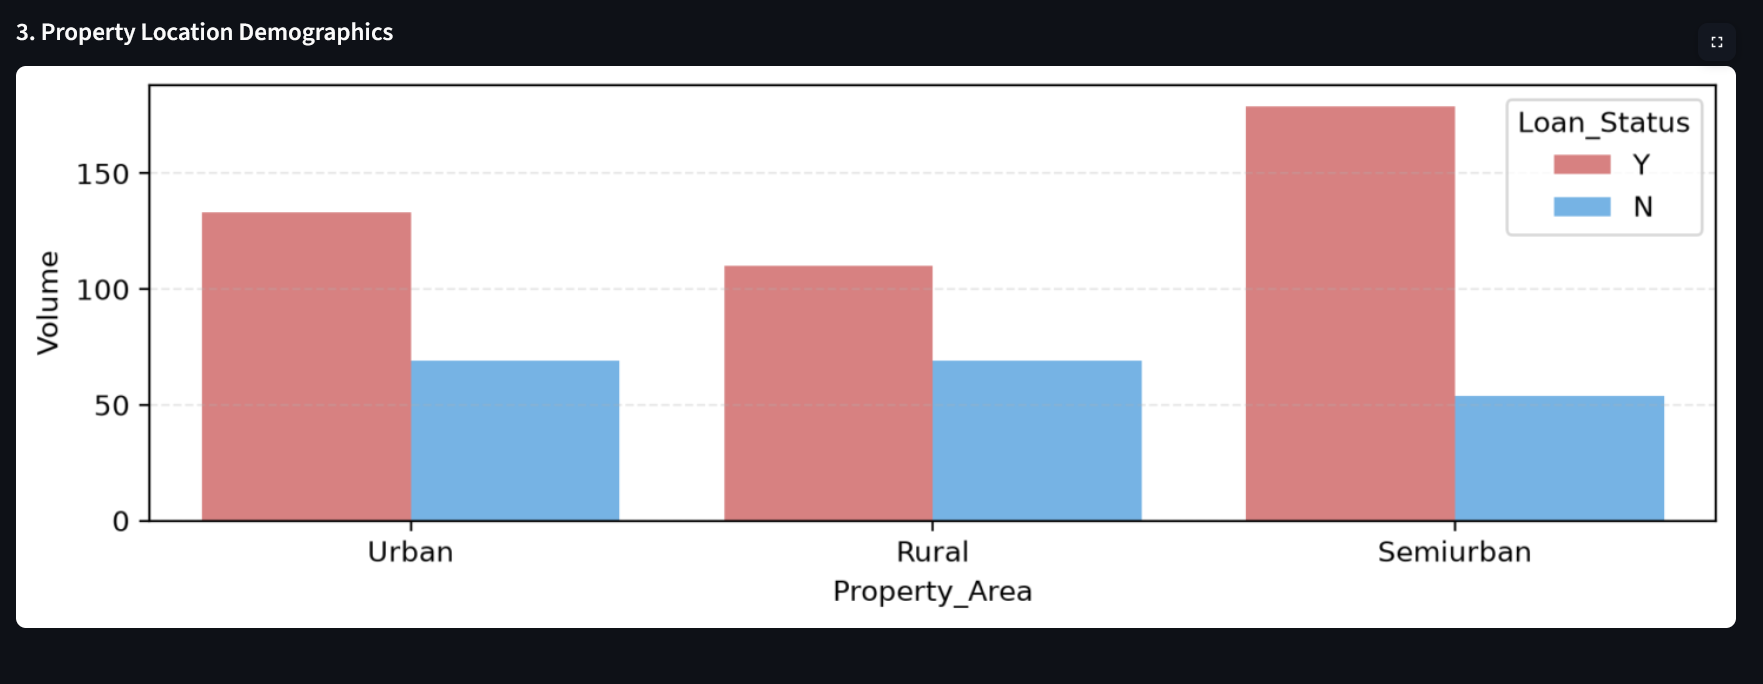
\includegraphics[width=0.72\linewidth]{fig3_demographics.png}
    \caption{Property Location Demographics showing approval distribution across Urban, Rural, and Semiurban zones.}
    \label{fig:demographics}
\end{figure}

As shown in Figure~\ref{fig:demographics}, Semiurban applicants achieved the highest overall approval volume and rate (76.8\%), while Rural applicants had the lowest (61.5\%). Because mean income and credit-history rates remain broadly comparable across zones, this regional variance is reported descriptively rather than attributed to a single observed causal driver.

\clearpage

% =============================================================
% PAGE 4: MACHINE LEARNING DIAGNOSTICS & BENCHMARKS
% =============================================================

\section{Machine Learning Architecture \& Diagnostics}
An ensemble \textbf{Random Forest Classifier} ($n=120$ estimators, $\text{max depth}=5$, balanced class weighting) was coupled with \texttt{SimpleImputer} inside a Scikit-Learn \texttt{Pipeline} using an 80/20 stratified split.

\begin{figure}[H]
    \centering
    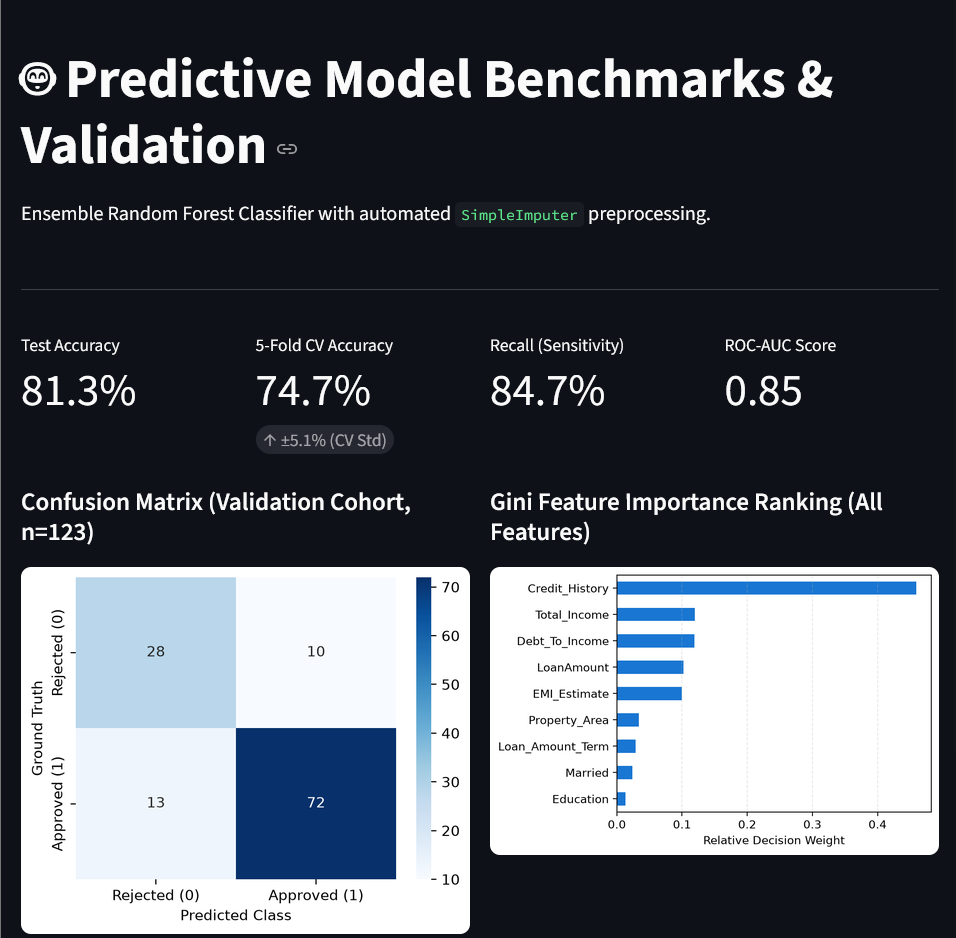
\includegraphics[width=0.78\linewidth]{fig4_model_diagnostics.png}
    \caption{Model Diagnostics: Holdout Benchmarks, 5-Fold Cross-Validation, Confusion Matrix, and Gini Feature Importance.}
    \label{fig:diagnostics}
\end{figure}

\subsection{Performance Validation \& Baseline Lift}
In this cohort, a naive majority-class rule (approving all applicants) yields a 68.7\% baseline accuracy. The model was evaluated using both 5-Fold Stratified Cross-Validation and an out-of-sample holdout test set ($n=123$):

\vspace{0.15cm}

\begin{itemize}
    \item \textbf{5-Fold Stratified Cross-Validation:} \textbf{74.7\% $\pm$ 5.1\%} (\textbf{+6.0 percentage points} above the 68.7\% naive baseline).
    \item \textbf{Holdout Validation Accuracy:} \textbf{81.3\%} ($100 / 123$).
    \item \textbf{Precision (Approval Class):} \textbf{87.8\%} ($72 / 82$).
    \item \textbf{Recall (Sensitivity):} \textbf{84.7\%} (Correctly identifying 72 of 85 approved cases).
    \item \textbf{ROC-AUC Score:} \textbf{0.85} (Strong class separation).
\end{itemize}

\vspace{0.15cm}

The Confusion Matrix confirms 72 True Positives, 28 True Negatives, 10 False Positives, and 13 False Negatives ($n=123$). The Gini Feature Importance confirms that \texttt{Credit\_History} accounts for over \textbf{45\%} of the decision weight, followed by continuous indicators \texttt{Total\_Income} (Rank 2), \texttt{Debt\_To\_Income} (Rank 3), \texttt{LoanAmount} (Rank 4), and \texttt{EMI\_Estimate} (Rank 5). Credit history provides the primary baseline separation, while the engineered ratios refine predictions on borderline applications.

\clearpage

% =============================================================
% PAGE 5: SIMULATOR, FAIRNESS & OPERATIONAL ROUTING
% =============================================================

\section{Underwriting Simulator \& Fairness Checks}
The trained pipeline was deployed inside a single-file \textbf{Streamlit Underwriting Simulator} to evaluate live applicant scoring.

\begin{figure}[H]
    \centering
    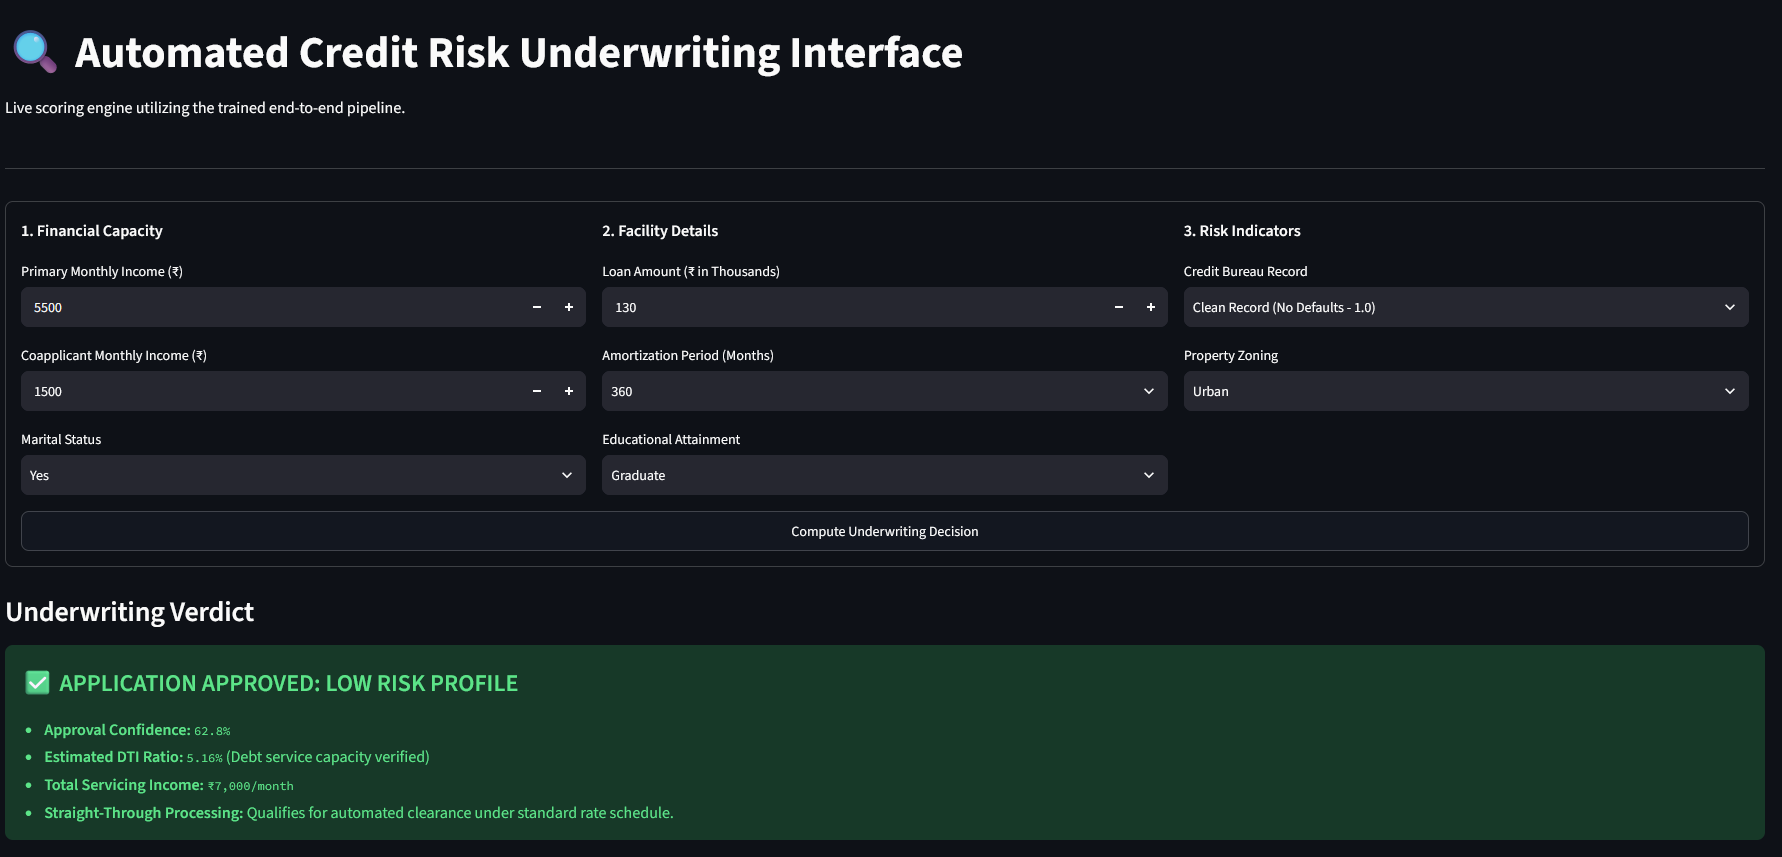
\includegraphics[width=0.72\linewidth]{fig5_simulator.png}
    \caption{Streamlit Underwriting Simulator displaying input fields and model approval verdict.}
    \label{fig:simulator}
\end{figure}

\subsection{Descriptive Fairness Check (UN SDG 10)}
To evaluate demographic parity in historical data, approval rates were checked across gender groups:

\begin{figure}[H]
    \centering
    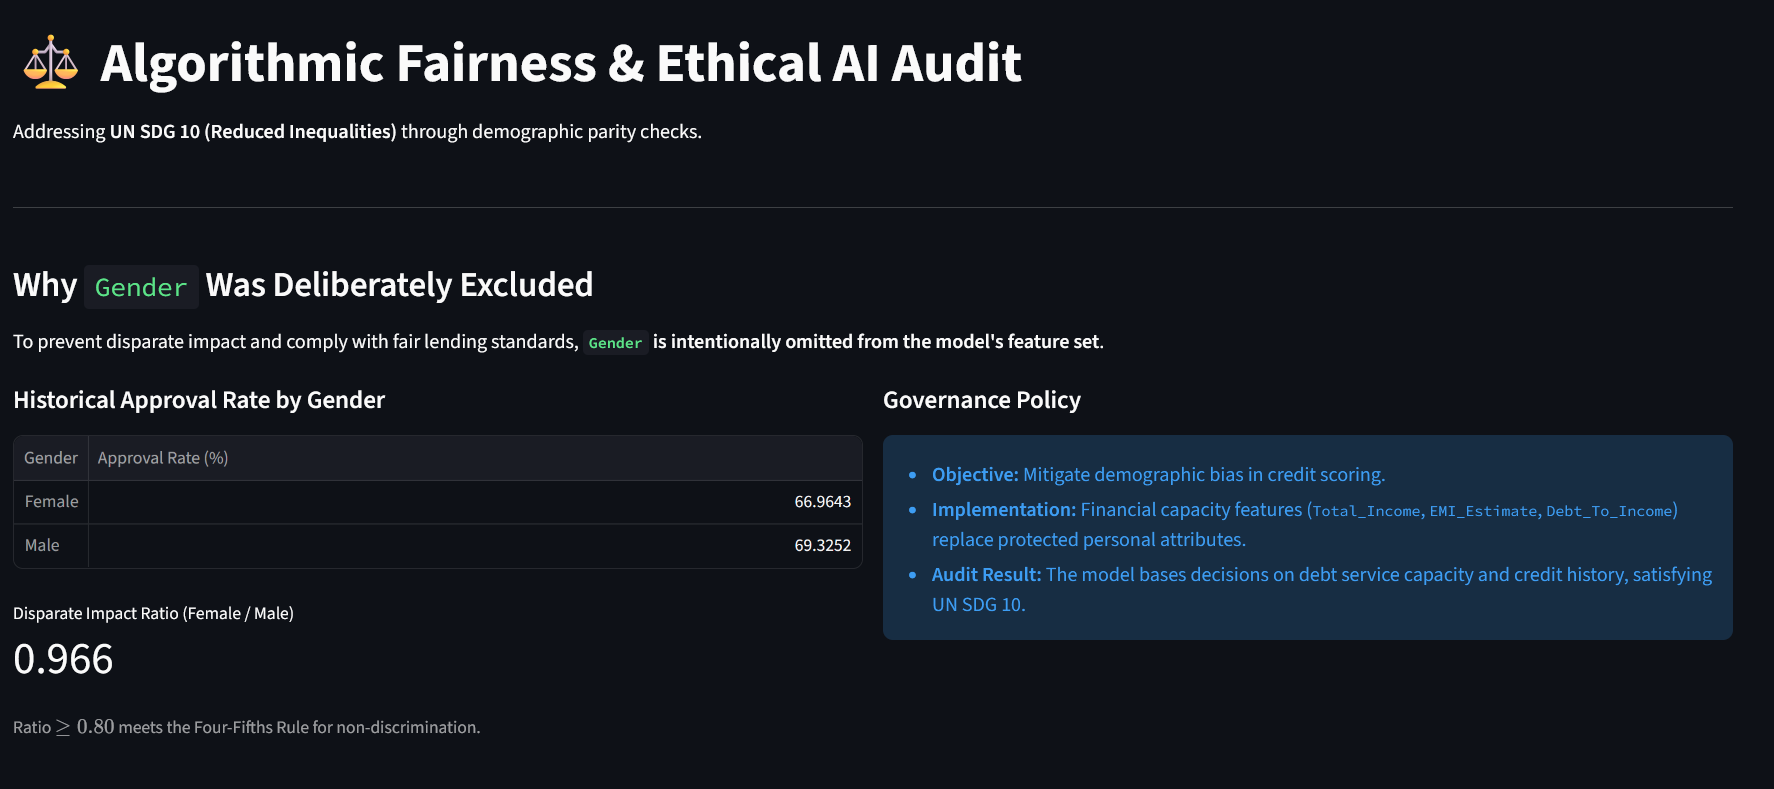
\includegraphics[width=0.72\linewidth]{fig6_Fairness_audit.png}
    \caption{Descriptive Fairness Check: Historical approval distributions and female-to-male ratio calculation.}
    \label{fig:fairness}
\end{figure}

As shown in Figure~\ref{fig:fairness}, the historical approval ratio between female (66.96\%) and male (69.33\%) applicants is \textbf{0.966}, satisfying the standard 0.80 Four-Fifths regulatory benchmark. Omitting \texttt{Gender} from the feature matrix ensures predictions remain anchored to creditworthiness and debt-service capacity.

\subsection{Operational Routing Framework (Illustrative Policy)}
To translate model probabilities into practical underwriting workflows rather than relying on a rigid 50\% cutoff, lending teams can deploy tiered risk bands. The cutoffs below represent an illustrative policy template:

\vspace{0.15cm}

\begin{enumerate}
    \item \textbf{Tier 1: Straight-Through Clearance:} High-confidence applications ($\ge 62\%$ approval probability) with verified clean credit records can receive automated first-pass clearance.
    \item \textbf{Tier 2: Secondary Committee Review:} Borderline applications ($50\% - 61.9\%$ probability) or cases with high debt-to-income ratios can be routed for manual underwriter review and collateral verification.
    \item \textbf{Tier 3: Elevated Default Risk:} Applications scoring $< 50\%$ are flagged for automated decline or restructuring under alternative lending terms.
\end{enumerate}

\clearpage

% =============================================================
% PAGE 6: LIMITATIONS, REPRODUCIBILITY & REPOSITORY
% =============================================================

\section{Limitations, Reproducibility \& Code Repository}

\subsection{Limitations \& Future Work}
This prototype is a learning exercise built on a small, single-source benchmark and has scope that a production deployment would need to extend:

\vspace{0.15cm}

\begin{itemize}
    \item \textbf{Sample size:} 614 records is small for subgroup fairness analysis; the female-to-male approval ratio (Section~5.1) is a useful descriptive signal but not a statistically robust guarantee at this sample size.
    \item \textbf{Fairness scope:} The current check compares only aggregate approval rates by gender. A production audit would additionally need equalized-odds and calibration checks (false-positive/false-negative rates by subgroup), and a review for proxy variables that could indirectly encode \texttt{Gender}.
    \item \textbf{Threshold calibration:} The routing tiers in Section~5.2 are an illustrative template, not thresholds derived from a validated precision-recall curve. Before operational use, they would need to be calibrated against business-specific cost tradeoffs between false approvals and false declines.
    \item \textbf{Generalization:} The dataset reflects a single historical lending cohort; performance on a different applicant population, geography, or time period is untested.
\end{itemize}

\subsection{Reproducibility}
The complete pipeline code, dataset references, dependencies, and execution logs are hosted publicly on GitHub, enabling independent verification of every metric reported in Section~4:

\begin{center}
    \textbf{Repository URL:} \url{https://github.com/Srijan9073/ibm-skillsbuild-analytics-capstone}
\end{center}

\subsection{Submission Deliverables Summary}
\begin{itemize}
    \item \textbf{Code File:} \texttt{app.py} --- integrated preprocessing pipeline, model training, and Streamlit interface.
    \item \textbf{Verification Script:} \texttt{scripts/verify\_metrics.py} --- reproduces the reported cross-validation and holdout metrics independent of the dashboard.
    \item \textbf{Dependencies:} \texttt{requirements.txt} (direct dependencies) and \texttt{requirements.lock} (full frozen environment).
    \item \textbf{Dataset Source:} Kaggle Open Benchmark (\texttt{train\_loan\_data.csv}), 614 records, 12 attributes.
    \item \textbf{Candidate:} Srijan Das (Internship ID: \texttt{IBMUEDA0483}).
\end{itemize}

\end{document}